\documentclass[10pt,twocolumn]{article} 
\usepackage{simpleConference}
\usepackage{times}
\usepackage{graphicx}
\usepackage{amssymb}
\usepackage{url,hyperref}
\usepackage{amsmath}

%caption loading 
\usepackage{caption3}
\DeclareCaptionOption{parskip}[]{} 
\usepackage[small]{caption}

\begin{document}
\title{Examining Phylogenetic Reconstruction Algorithms}

\author{}

\maketitle
\thispagestyle{empty}

\section*{Multiple Sequence Alignment Algorithms}
\subsection*{ClustalW}
In order to reconstruct phylogenetic trees from multiple sequences of different lengths, the sequences need to be aligned first to allow for accurate similarity measures. ClustalW is such an algorithm for multiple sequence alignment (MSA). Introduced in 1994, considered to be a progressive alignment algorithm, it represented dramatic progress in alignment sensitivity combined with other existing tools, and is still the most widely used MSA program \cite{edgar2006multiple}. There are three main steps of the algorithm:
\begin{enumerate}
  \item \textbf{The Distance Matrix/Pairwise Alignment.} This is done using dynamic programming as a standard practice \cite{thompson1994clustal}. Optimal alignment is guaranteed with this approach given a table of scores for matches and mismatches  between sequence characters and penalties for insertions or deletions. The scores of each pair of alignments are then calculated using the Sum-of-pairs (SP) measure, and a distance matrix is constructed based on these scores.
  \item \textbf{Create a Guide Tree.} The trees used to guide the multiple sequence alignment are calculated from the distance matrix of step 1 using Neighbor-Joining. 
  \item \textbf{Progressive Alignment Using the Guide Tree.} This final stage is done using a series of pairwise alignments to align progressively larger groups of sequences following the branching order in the Guide Tree we created in the second step, starting from the tips of the rooted tree towards the root terminating in the completed MSA. \cite{thompson1994clustal}.
\end{enumerate}
\subsubsection*{Merits}
The main advantage of the progressive strategy used by ClustalW is its speed and relative robustness \cite{notredame2000t}. \\

ClustalW also requires much less memory than other programs. Therefore, it is suggested that it should be used on aligning small number of unusually long sequences \cite{edgar2006multiple}.\\

\subsubsection*{Critiques}
As one of the mostly widely used MSA program, ClustalW has been improved through better decision making process during multiple alignment (e.g. when to change weight matrix) and the accuracy and appropriateness of parameterization. However, no significant improvements have been made since 1994 and several modern methods (e.g. MAFFT, MUSCLE, T-COFFEE) achieve better performance in accuracy, speed or both \cite{edgar2006multiple}.\\

Although widely used in a variety of cases, ClustalW suffers from its greediness as errors made in initial alignments cannot be corrected later as the rest of the sequences are added in \cite{tamura2004prospects}. In addition, there is no way of quantifying whether the resulting alignment is good, or if the alignment is correct due to the algorithm's greedy nature.\\

\subsection*{MUSCLE}
As the exploration of phylogenetic reconstruction has advanced, so too has the desire for highly accurate alignments. MUSCLE is an approach strikingly similar to ClustalW with some modifications made to quickly reach the alignment phase. Introduced in 2004 MUSCLE has been gaining traction among the various MSA's for its use on alignments of large data sets of short sequences. MUSCLE has three main phases:
\begin{enumerate}
  \item \textbf{Draft Progressive} The first iteration focuses on speed over accuracy, quickly transforming the raw sequences into sloppily aligned sequences.
  \begin{enumerate}
  	\item \textbf{kmer Distance} A distance matrix is produced by converting the basic sequences to their amino acid sequences. From there each sequence is given an identity of the frequencies of k-tuples in the amino acid chain. Euclidean distance is used on the series of frequencies to determine relations amongst the sequences.
  	\item \textbf{Guide Tree 1} Using a heuristic to cluster the sequences, the guide tree is formed. In this case, neighbor joining.
  	\item \textbf{Progressive Alignment} The alignments are produced identically to ClustalW with the exception that a differing scoring system is employed with the goal of accounting for gaps in sequences more accurately.
\end{enumerate}
  \item \textbf{Improved Progressive} Now that the sequences are aligned, the process will be repeated using a different metric to improve the alignments.
    \begin{enumerate}
  	\item \textbf{Kimura Distance} Every distance between sequences is computed using the Kimura metric. Essentially the distance becomes how many matching characters each sequence shares.
  	\item \textbf{Guide Tree 2} The guide tree is reproduced on the new distances in the same manner as before.
  	\item \textbf{Progressive Alignment} The alignment process is repeated here as well, with the opportunity to only realign on sections of the new guide tree that differ from the old one to cut down on processing time.
\end{enumerate}
  \item \textbf{Refinement} Here is where MUSCLE diverges most from ClustalW. Visiting an edge we cut the tree into two subtrees, realigning their profiles individually, reconnecting them, and realigning as a whole.  If the action has netted an improvement the change is kept, otherwise the refinement is considered to be done. This process is repeated until convergence or user satisfaction.
  \end{enumerate}
  
\subsubsection*{Merits}
MUSCLE is best for large sets on the order of a hundred species with short lengthed sequences, where the process of eliminating the initial pairwise alignment outweighs the cumbersome refinement process.

Easily the most defining feature of MUSCLE vs ClustalW is the refinement period which tackles the weak exploration of ClustalW which should lead to more accurate alignments.

\subsubsection*{Critiques}
While some improvements have been made over the basis of clustalW the refinement phase is still terribly expensive to run, with little garauntee of dramatic improvement. The refinement phase caps the performance at an $O(n^3L^2)$. operation

\subsection*{Center Star}
Center Star is a method which does not use tree or clustering methods in constructing a multiple sequence alignment. Instead center star identifies the most "central'' sequence which when aligned to every other sequences has the lowest total distance between itself and all other sequences. This method is by far the simplest and near the fastest of the mentioned algorithms, and can be shown to produce an alignment no worse than two times the optimal alignment's total distance. Center star operates as follows:
\begin{itemize}
\item \textbf{Center Sequence Identification} By computing an n x n matrix of the hamming distance between each sequence and finding the sequence which minimizes this value, the center of the alignments can be found.
\item \textbf{Center Sequence Matching} Every sequence is pairwise aligned to the center sequence.
\item \textbf{Combination} By combining the center sequences between each pair alignments that have been aligned uniquely we can find the conglomerate sequence, which gains the spacing of both it's component center sequences. From there we align the matched sequences to the conglomerate and repeat until all the sequences have been combined into a multiple alignment.
  \end{itemize}
\subsubsection*{Merits}
Center Star is easy to create and runs in $O(n^2L^2)$.

\subsubsection*{Critiques}
The algorithm can be described as a "quick and dirty'' method of generating a multiple alignment with no garauntee that it's entirely optimal.


\section*{Tree Reconstruction Algorithms}
\subsection*{Neighbor Joining Method}

Reconstruction of phylogenetic trees generally involves inference of phylogenies consisting of large amounts of gene sequences. First proposed by Naruya and Masatoshi \cite{saitou1987neighbor} the neighbor-joining (NJ) method is frequently used to construct phylogenetic trees of life because of its known accuracy and relatively fast computational speed. The use of neighbor-joining is so wide spread, in fact, that it has become a common baseline to compare newly proposed reconstruction algorithms to \cite{mihaescu2009neighbor}.\\

Neighbor joining itself is a very simple algorithm. First, a distance metric is used to compute pair-wise distances between all possible pairs of input sequences, a common practice in so-called ``distance matrix'' methods. Based on this distance matrix, a similarity metric is used to find the two most similar sequences, which can be thought of as nodes in the eventual phylogenetic tree. Once discovered, these two sequences, now considered as leaf nodes, are connected by a common parental node. The distance between this new parental node and all other nodes represented in the distance matrix is estimated. This process continues, until there are only two nodes remaining. At this point, the algorithm has greedily and hierarchically constructed a phylogeny.

\subsubsection*{Merits}

Tamura, Nei, and Kumar demonstrated the accuracy of NJ trees for inferring very large phylogenies using the reports of their computer simulations \cite{tamura2004prospects}. Given pairwise distances estimated using biologically realistic models of nucleotide substitution, reports show that the accuracy of NJ trees decline only by about $5\%$ when the number of sequences used increases from 32 to 4,096 (128 times) even in the presence of extensive variation in the evolutionary rate among lineages or significant biases in the nucleotide composition and transition/transversion ratio. These results suggest the promising prospects for inferring large phylogenies using the NJ method.\\

Furthermore, the use of the NJ method has some appealing theoretical guarantee. Atteson shows that, for appropriately long and accurate multiple sequence alignments, NJ will produce the correct phylogeny for certain data; a formal bound is provided for the requirements of the inputs \cite{atteson1999performance}. Though this is an important result regarding the theoretical guarantee of this algorithm, the formal conditions required for data inputs are often not met in practice, though NJ still performs exceptionally well. Mihaescu et al. \cite{mihaescu2009neighbor} provide an extension of Attesons theorem that explains this apparent discrepancy, and quantify the usefulness of NJ in practice.

SOMETHING ABOUT RUNTIME.

\subsubsection*{Critiques}
A distance-based method, NJ has the disadvantage of discarding the actual character data in the sequences \cite{brinkman2001phylogenetic}. Since it is designed to produce only one tree, it can obscure ambiguities in data. Although ambiguities can be uncovered by using resampling methods, if used alone, NJ programs may give misleading bootstrap frequencies because they do not suppress zero-length branches and/or are sensitive to the order of terminals in data. In addition, resampling can be employed with parsimony methods, which are far more efficient than NJ methods \cite{farris1996parsimony}.

\subsection*{Maximum Parsimony}
Maximum Parsimony is another method used for inferring phylogenies. ``The maximization of parsimony'', or preferring the simplest of otherwise equally adequate theories is the guiding principle in this method. With the assumption that evolution is inherently a parsimonious process, Maximum Parsimony values phylogenetic trees where the least evolution is required to group taxa together \cite{fitch1971toward}.

To find the maximum parsimony tree given a data set is equivalent to solving two sub-problems: constructing a list of all possible trees and to determine the length of each given tree.

Since the number of possible trees grows tremendously rapidly with the the number of species, it is not possible to do an exhaustive search of all trees. Thus a heuristic approach is taken:
\begin{enumerate}
\item Construct initial tree and determine its length.
\item Construct a set of ``neighboring trees'' using Nearest Neighbor Interchange.
\item If any of the neighboring trees are better than the initial tree, then select it/them and use as starting point for new round of rearrangements.
\item repeat steps 2 and 3 until a tree that is better than all of its neighbors is found. This tree is a ``local optimum''.
\end{enumerate}

To determine the length of a given tree, the Fitch Algorithm is used.
\begin{enumerate}
\item Root the tree at an arbitrary internal branch.
\item Visit an internal node x for which no state set has been defined, but where the state sets of x's immediate descendants (y,z) have been defined.
\item If the state sets of y,z have common states, then assign these to x.
\item If there are no common states, then assign the union of y,z to x, and increase tree length by one.
\item Repeat until all internal nodes have been visited and return the length of the current tree.
\end{enumerate}

\subsubsection*{Merits}
The principle of constructing a maximally parsimonious tree takes advantage of Occam's razor, which, in this context, states that the topology which assumes the least amount of total evolutionary events is the most likely to occur. Because mutations are relatively unlikely, the tree of ``minimal evolution'' is likely a good approximation of the actual evolutionary history of a a system.

The principles guiding the Maximum Parsimony approach frees the algorithm from making other assumptions, unlike other models used in phylogenetic reconstructions.

(Something more relevant here)

Furthermore, Fitch's algorithm lends itself exceptionally well to parallelization. Because a ``read-only'' tree traversal must be executed for each site in a genome, according to Gustafson's Law of parallelization, the speedup we can achieve on this portion of the program is exactly equal to the number of processors we have available, because no sequential operations must take place. Depending on the size of the topology and the length of the genomes, either a multi-core CPU or GPGPU implementation might be effective.

\subsubsection*{Critiques}
Unfortunately, evolution is not a completely parsimonious process, though it is assumed to be in Fitch's original method. Unlikely events, which can cause massive change to occur in genomic sequences, do occur in organic evolution. For instance, gene duplication is a type of mutation that causes multiple copies of DNA segments to be re-inserted into the original genome. Assuming such a mutation is surely not the most likely explanation for evolution in some cases, but it occurs nonetheless.

Fitch's original algorithm for determining the minimum number of mutations for a given topology does not produce edge weights. In other reconstruction algorithms, edge weights offer a sense of evolutionary distance, and this information is simply not present in topologies reconstructed using parsimony methods. (check to see if there are any parsimony-based edge-weight generating algorithms)

Maximum Parsimony is not a statistically consistent method in finding the true best tree given sufficient data. Consistency refers to the monotonic convergence on the correct answer with the addition of data, and Maximum Parsimony lacks this consistency under the category of situations called ``long branch attraction'' \cite{felsenstein1978cases}. Under these situations, there are high levels of substitutions for two characters and low levels of substitutions for others. The more data we collect, the more we tend towards finding the wrong tree.

In addition, because Maximum Parsimony uses heuristic methods in searching tree space, the most parsimonious tree is not guaranteed to be obtained. However, this problem is not unique to this algorithm; any algorithm that uses an optimality criterion is subject to the same critique.


\subsection*{Maximum Likelihood}

Reconstruction of a phylogenetic tree with a maximum likelihood approach was first proposed by Felsenstein in 1981 [1]. The recent advancement in computational power has overcome its disadvantage of high computational cost, and the maximum likelihood approach became one of the most popularly used methods of phylogenetic reconstruction. In more recent history the maximum likelihood approach has been used to uncover the confounding evolutionary history of some species, such as the giant panda and dolphins [2][3][4]. 

The core concept of the maximum likelihood approach is to find a phylogeny tree that has the highest likelihood of obtaining an observed set of DNA sequences. Note that the likelihood of a tree is the probability of a given tree yielding the observed outcome; it is not the probability of a tree being the correct one [1] .
 
\subsubsection*{Assumptions}
The maximum likelihood approach makes three assumptions to make computation faster and easier [1].
\begin{enumerate}
  \item Nucleotide substitution happens site independently. This means that the mutation rate of a nucleotide at one location is not affected by any other nucleotide at a different location. 
  \item Two lineages evolve independently after speciation. In other words, any pair of two species will not affect the evolutionary processes of each other.
  \item Any lineage has the same probability of nucleotide base substitutions. For example, if species A had 20 percent chance of cytosine mutating to thymine, the same rate applies to species B.
\end{enumerate}

\subsubsection*{Likelihood calculation}
By the first assumption of site-independent evolution, the likelihood of an entire tree can be calculated by computing the likelihood values site by site, and multiplying them all together. The likelihood of a tree at one DNA site is then calculated by multiplying the probability of each segment of a tree and the prior probability of the root [Figure 1]. The probability of a tree segment is computed using the segment length, mutation rates, and the nucleotide bases of the two nodes in the segment. We do not know the nucleotide bases of the internal nodes, since they represent common ancestors that are now extinct. To account for this, the likelihood is computed as the sum of all possible assignments of nucleotide bases to the internal nodes [1]. The following equation computes the likelihood of the tree in ~\ref{fig:ml}.

\begin{align*}
L = & \sum\limits_{s_0}  \sum\limits_{s_6}  \sum\limits_{s_7}  \sum\limits_{s_8} \pi_{s_0} P_{s_0 s_6}(v6) P_{s_0 s_6}(v6) P_{s_6 s_1}(v1) 
\\ & P_{s_6 s_2}(v2) P_{s_0 s_8}(v8) P_{s_8 s_3}(v3) P_{s_8 s_7}(v7) P_{s_7 s_4}(v4)
\\ & P_{s_7 s_5}(v5)
\end{align*}
where $P_{s_x s_y}(v)$ denotes the probablity of a nucleotide $s_x$ changing to $s_y$, given branch length $v$.

\begin{figure}
\begin{centering}
  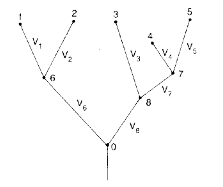
\includegraphics{media//ml.png}
  \caption{An example tree for likelihood calculation. This figure is taken from the paper written by Feslenstein 1981}
  \label{fig:ml}
\end{centering}
\end{figure}

\subsubsection*{Topology searching}
Our objective is to use equation 1 to calculate the likelihood of a tree and to find a tree that yields the highest likelihood of obtaining the observed dataset. It is simply impractical to compute the likelihood values of all possible topologies with all possible branch length. In this  study, we implemented two types of tree searching algorithm. \\

The first approach is an heuristic approach that begins with a tree with two randomly chosen species[1]. Every iteration, you add one species to every segment of the tree, thereby creating 2k-5 topologies for the kth species being added to the tree. Each topology will have its branch length adjusted so that it yields the highest possible likelihood with that topology. Finally, the topology with the maximum likelihood will make it to the next iteration. These steps are repeated until all of the species in the observed data set are added to the tree. \\

The second approach starts with a randomly constructed tree with all species in the DNA dataset[6]. We check the neighborhoods of the current tree by swapping subtrees of every internal edge. This procedure is repeated until a better tree can no longer be found in the neighborhood of the current tree. The same tree searching method is used in the neighbor joining approach. The former method runs significantly faster due to its smaller topology search space. However, the outcome of the algorithm will depend on the order of addition of the species. On the other hand, the latter method produces a tree that is independent of the order of addition, but the run time is significantly larger due to its large search space. \\

\subsubsection*{Merits and Critiques} 

While the maximum likelihood method produces more accurate trees compared to other reconstruction methods, it is computationally costly mainly due to the likelihood calculations in the branch optimization process. The big-O runtime of the algorithm is $O(mn^6)$ with the progressive topology and $O(kmn^5)$ with the hillclimb approach, where $k$ is the number of hillclimb iterations, $m$ is the length of DNA sequences, and n is the number of species. The maximum likelihood algorithm also assumes that the nucleotides mutate site-independently, and thus, it does not accurately account for changes such as insertion or deletion. Commonly accepted solutions to this indel probelm are (i) remove all sites in which any gap appears, (ii) assign an imaginary nucleotide for gaps, and (iii) treat gaps as missing data. In this project, we used the option (ii), as Evans et al showed that the option (iii) can have deleterious effects on the reconsturnction [5].  

\subsection*{Markov Chain Monte Carlo for Bayesian Analysis}
Traditional methods for phylogenetic inference select a single ``best'' tree, while a Bayesian approach expresses the uncertainty in phylogeny and in the parameters of the sequence mutation model with a posterior probability distribution \cite{larget1999markov}. The computational aspects of the problem can be efficiently solved by the Markov Chain Monte Carlo (MCMC) algorithms.

MCMC technique was first introduced by Yang and Rannala in 1997 \cite{yang1997bayesian}. It was later developed by Mau, Newton, and Larget \cite{mau1999bayesian}. We adopted a simplified version from Larget and Simon \cite{larget1999markov}. In their original paper, they presented two MCMC algorithms: $GLOBAL$, in which all branch lengths in topologies are adjusted with every cycle, and $LOCAL$, which allows for the same changes but with different probabilities. After an initial burn-in period, the Markov Chain runs for 2,000 cycles with $GLOBAL$ followed by $LOCAL$ to complete tree paremeter proposals and outputs the final tree. We implemented both algorithms under the molecular clock assumption.

\subsubsection*{Metropolis-Hastings Algorithm}
The Metropolis-Hastings algorithm (M-H) is used to sample a dependent sequence of points such that after some point in the sequence, all subsequent sampled points are distributed approximately according to the posterior distribution \cite{larget1999markov}. Therefore, the long-run frequencies of sampled tree topologies are arbitrarily close to their posterior probabilities after sufficiently long simulations. M-H is used in constructing the Markov chain on tree parameters (topologies and associated branch lengths). The Markov chain proposes a move to state $\omega_2$ from the current state $\omega_1$ according to probability density function $q(\omega_1,\omega_2)$. If the new state is rejected, the current state is repeated in the sequence. M-H modifies these transition probability densities so that the resultant stationary distribution is the desired posterior distribution.

\subsubsection*{$GLOBAL$ with a Molecular Clock}
This algorithm changes all branch lengths with every cycle. Under the molecular clock assumption, the pair of distances to adjacent leaves are maintained to be equal for each internal node.
\subsubsection*{$LOCAL$ with a Molecular Clock}
This algorithm modifies the tree only in a small neighborhood of a randomly chosen internal branch, and each different modification is made with different probabilities. It is also implemented under the molecular clock assumption.


\subsubsection*{Merits and Critiques}
Compared to Yang and Rannala's approach (\cite{yang1997bayesian}), this algorithm can work with much larger trees. It generates a posterior distribution of phylogenetic trees, giving it substantial advantages over traditional maximum likelihood algorithms. In addition, the calculation of an acceptance probability of a proposed tree sums over the unknown data at the internal nodes, a rapid and accurate process with pruning algorithm (\cite{felsenstein1983statistical}).
Since MCMC depends on the underlying likelihood model, data sequences generated by the best fitted model would likely differ from geniune data regarding composition of amino acids, locations of stop codons, and other biologically relevant features (\cite{larget1999markov}).
A more fundamental problem underlying an MCMC algorithm is its ability in correctly identifying the posterior probabilities of the collection of highly probable tree topologies. It is difficult for a particular simulation to visit new regions of parameter space once it gets stuck in an old region (\cite{larget1999markov}). Likewise, it is relatively difficult to transition between islands of high posterior probabilities. Thus, this model may often yield inconsistent results when applied to the same sets of data.


\section*{Tree Comparison Algorithms}
In order to properly compare alignment and reconstruction methods, we require methods of comparing their ultimate outputs. We decided to use two different tree-distance metrics; one focused on absolute distance between species that utilized branch lengths, and one concerned with overall tree topology. Together, we believe these metrics summarize the differences and similarities between trees effectively. Note that these two metrics are part of a larger class of comparison methods known as ``dissimilarity metrics;'' this means that higher values indicate greater dissimilarity.

\subsection*{Quartet Distance: Topological Metric}
\begin{figure}
\begin{centering}
  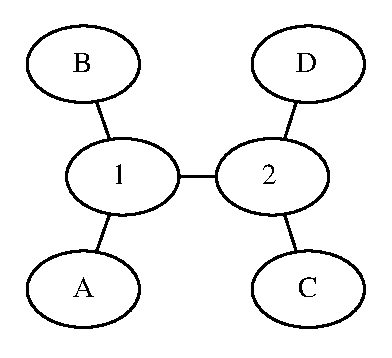
\includegraphics{media//quartet.eps}
  \caption{An example of a quartet, denoted as $AB|CD$.}
  \label{fig:quartet}
\end{centering}
\end{figure}
To compare the similarity of topologies numerically, we employ a ``quartet'' based method, first proposed for this purpose by Estabrook, McMorris and Meacham \cite{estabrook1985comparison}. A quartet is a phylogenetic tree with only four species, divided by two internal nodes as in Figure ~\ref{fig:quartet}. To ``reduce'' a phylogeny to a quartet given four species, first, remove all non-desired species from the tree. Next, remove edges and internal nodes shifting your remaining species appropriately until you are left with only a quartet. This quartet should maintain structural properties of the original tree; the remaining species now represent reductions of subtrees in their original topological formations. Computing a phylogenetic reduction is $O(n)$ because it requires a single traversal of the tree. Many previous studies have employed quartet distance as a means of analyzing the similarity of phylogenetic topologies in both theoretical an practical settings. For instance, Puigbo et al. \cite{puigbo2010tree} utilize this metric in their analysis of horizontal gene transfer in prokaryote evolution

To compute the quartet-distance between any two topologies, say $T_1$ and $T_2$, that contain the same $n$ species, we compute all size-4 subsets $\{a,b,c,d\}$ of the $n$ species and count the number of times the reduction of $T_1$ to $\{a,b,c,d\}$ doesn't match the reduction of $T_2$ to $\{a,b,c,d\}$. The brute force algorithm, as described, is $O(n^5)$ because there exist $O(n^4)$ size-4 subsets of the $n$ species, and for each subset, two $O(n)$ reductions must be computed.

Fortunately, there exist algorithms that reduce the time complexity of this computation significantly; Brodal et al. \cite{brodal2004computing} present an $O(nlogn)$ solution to the quartet-distance problem, which represents the current state-of-the-art. For our purposes, we utilize a simpler $O(n^3)$ solution, originally proposed by Christiansen et al. \cite{christiansen2005computing}.

Central to this improved algorithm is the fact that, given any three species $\{a,b,c\}$ within a bifurcating phylogeny, there is exactly one internal node such that the paths between $\langle a, b \rangle$, $\langle b, c \rangle$, and $\langle a, c \rangle$ intersect at that node. Deleting such an internal node and its incident edges would result in three subtrees, each containing one of $a$, $b$, and $c$. Denote the subtrees as $T^a$, $T^b$, and $T^c$. For each species $x \in T^a - \{a\}$, we can determine that the quartet of our original tree restricted to $\{a,b,c,x\}$ will be $ax|bc$. Symmetric principles apply to $T^b$ and $T^c$. While further algorithmic detail is not necessary, this is the primary observation that allows us to reduce our time complexity to $O(n^3)$, as we now restrict our consideration to speices subsets of size three.

\subsection*{Pairwise Path Distance: Branch Length Metric}
Because quartet distance doesn't account for branch lengths and many of our tree reconstruction algorithms produce weighted topologies, a secondary metric that accounts for this additional information is required. First proposed by Williams and Clifford \cite{williams1971comparison}, we utilize a version of pairwise pathlength distance similar to that proposed by Steel and Penny \cite{steel1993distributions}. The focus of this comparison method is computing all the pathlength between all pairs of species in a given phylogeny.

More specifically, pairwise pathlength distance can be computed as follows. Given two trees with associated branch lengths $T_1$ and $T_2$ each containing species $\{S_1, S_2 \ldots S_n\}$, consider a fixed ordering of all possible species pairs $\langle (S_1, S_2), (S_1, S_3) \ldots (S_{n-1}, S_n) \rangle$. Consider $\vec{d_1}, \vec{d_2}$, the ordered pairwise pathlength distances between the species specified in the ordering for $T_1$ and $T_2$. After normalizing these vectors such that each of their largest components is equal to one, the pairwise path distance between $T_1$ and $T_2$, then, is given by

\begin{align}
  d_{path}(T_1, T_2) = ||\vec{d_1} - \vec{d_2}||_2
\end{align}

where $||\cdot||_2$ is the $L_2$ (Euclidean) norm.

The time complexity of this metric's computation is $O(n^3)$. For a given tree, there are ${n \choose 2} = O(n^2)$ pairs of species to compute the distance between, and each distance computation can be completed using an $O(n)$ breadth first search. Alternative approaches using algorithms like Floyd–Warshall \cite{floyd1962algorithm} which compute all pairwise pathlengths are possible. However, given the topological structure of our trees, namely that the total number of edges and nodes both grow linearly with the number of species, the simpler, proposed method has the same worst-case time complexity.

\section*{Experiments}

\subsection*{Methods}
\subsubsection*{Experiment 1}
Our random data generator is capable of producing testing examples $\langle T, D \rangle$ where
$T$ is a randomly generated phylogenetic tree containing $n$ species, and $D$ is a set of $n$ 
sequences generated based on that synthetic tree. We can use $D$ as input to total 18 combinations of 
the 3 multiple sequence alingment algorithms and the 6 reconstrunction algorithms, which will each output 
some tree $T'$. We can then use our two comparison functions to evaluate the relative distance between 
the true tree $T$ and the tree we produced $T'$.

\begin{enumerate}
  \item 14 test examples $\{\langle T, D \rangle\}$ with 4 species, 50 bps.
  \item 14 test examples $\{\langle T, D \rangle\}$ with 8 species, 50 bps.
  \item 14 test examples $\{\langle T, D \rangle\}$ with 12 species, 50 bps.
  \item 14 test examples $\{\langle T, D \rangle\}$ with 4 species, 500 bps.
  \item 14 test examples $\{\langle T, D \rangle\}$ with 8 species, 500 bps.
  \item 14 test examples $\{\langle T, D \rangle\}$ with 12 species, 500 bps.
  \item 14 test examples $\{\langle T, D \rangle\}$ with 4 species, 1500 bps.
  \item 14 test examples $\{\langle T, D \rangle\}$ with 8 species, 1500 bps.
  \item 14 test examples $\{\langle T, D \rangle\}$ with 12 species, 1500 bps.
\end{enumerate}

For each of these 9 experiments, we will be able to produce confidence intervals for how
accurate the reconstructed trees are for all methods, given our two distance metrics
(pairwise distance will be used to compare the 12 methods that produce branch lengths,
quartet distance will be used to compare the 18 methods that produce topologies). The average 
runtime of each of the 18 methods will aslo be recorded.

\subsubsection*{Experiment 2}
We have a dataset $\langle T, D \rangle$ where $T$ is the commonly accepted phylogeny
for 53 species (50 primates and 3 non-primates), and $D$ are the DNA sequences of the mitochondrial cytochrome c oxidase 
subunit 1 (COX1) of those apes. COX1 is a popular choice for phylogenetic reconsturnction 
because it is hightly conserved due to its involvement with aerobic respiration. 
We can use $D$ as input to our 12 tree reconstruction algorithms, which will each 
output some tree $T'$. We can then use our two comparison functions to evaluate the 
relative distance between the true tree $T$ and the tree we produced $T'$. To test 
different numbers of species in our tree, we can select random subsets of the 53 extant species for 
our tree builders to analyze.

\begin{enumerate}
  \item 14 test examples $\{\langle T, D \rangle\}$ with 4 species.
  \item 14 test examples $\{\langle T, D \rangle\}$ with 8 species.
  \item 14 test examples $\{\langle T, D \rangle\}$ with 12 species.
\end{enumerate}

For each of the above experimental sets, we will be able to produce confidence intervals for how
accurate the reconstructed trees are for all methods, given our two distance metrics
(pairwise distance will be used to compare the 2 methods that produce branch lengths,
quartet distance will be used to compare the 18 methods that produce topologies). We 
then compare the results of experiment 1 and 2 to answer the following questions. The average 
runtime of each of the 18 algorithms will aslo be recorded.

\begin{enumerate}
  \item Do the random data results match the real data results?
  \item Is our random model of evolution too simple? 
  \item Which algorithm performs fastest on the real data?
  \item Which algorithm produces the most accurate tree on the real data?
\end{enumerate}

\subsubsection*{Experiment 3}
We have the mitochondrial DNA sequence data for the following 12 genes of the 50 primates and 3 non-primates.
\begin{enumerate}
  \item Cytochrom c oxidase subunit 1 (COX1)
  \item Cytochrom c oxidase subunit 2 (COX2)
  \item Cytochrom c oxidase subunit 3 (COX3)
  \item NADH dehydrogenase subunit 1 (ND1) 
  \item NADH dehydrogenase subunit 2 (ND2) 
  \item NADH dehydrogenase subunit 3 (ND3) 
  \item NADH dehydrogenase subunit 4 (ND4)
  \item NADH ubiquinone oxidoreductase chain 4L (ND4L) 
  \item NADH dehydrogenase subunit 5 (ND5)
  \item ATP synthase F0 subunit 6 (ATP 6)
  \item ATP synthase F0 subunit 8 (ATP 8)
\end{enumerate}

We run the best performing reconstruction algorithm from experiment 2 on each gene, and 
investigate on how much resulting trees variate depending on which gene you choose to 
run the algorithm on. 

\begin{enumerate}
  \item Randomly select 20 species from the dataset.
  \item Run the best reconstruction algorithm on all mtchondrial DNA genes listed above.
  \item Measure the variation in resulting trees.
\end{enumerate}

\subsection*{Hypothesis}
We hypothesize that the method with Center Star and Neighbor Joining has the shortest average running
time on randomly generated data due to its algorithmic simplicity. We believe that Clustal W/Maximum Likelihood
and Clustal/Markov Chain Monte Carlo will perform better than other methods in terms of the accuracy of tree reconstrunction
on the random data. Similarly, in experiment 2, we expect to see Centar Star/ Neighbor Joining being dominant in terms of running time, and Clustal W/Maximum Likelihood and Clustal/Markov Chain Monte Carlo being dominant in terms of the accuracy of resulting trees.

For experiment 3, we hypothesize that resulting trees will variate significantly depending on which gene is inputted into the algorithm.  

\subsection*{Results}
\subsection*{Discussion}
\subsection*{Conclusion}

\bibliographystyle{abbrv}
\bibliography{refs}
\end{document}
